
\section{Introduction}

\begin{frame}[t]{Introduction}

Intro to gensim project and group

\end{frame}

\begin{frame}{Structure of the Tutorial}

\begin{itemize}
\item Talk 1: Introduction (1 Hour)
\begin{itemize}
	\item blah
	\item blah
\end{itemize}

\item Hands-On Session (90 Minutes)
\begin{itemize}
	\item blah
	\item blah
\end{itemize}

\item Talk 2: Building a Model (1 Hour)
\begin{itemize}
	\item blah
	\item blah
\end{itemize}

\end{itemize}

\end{frame}

\begin{frame}[t]{Instruction Set Simulation}

What is simulation? 

\end{frame}

\begin{frame}[t]{Instruction Set Simulation}
\vspace{0pt}
\begin{minipage}{\textwidth}
	\vspace{0pt}
	Instruction Set Simulation is used in a wide variety of contexts:
	\begin{itemize}
		\item<2-> Design Space Exploration
%		\only<2>{
%			\begin{itemize}
%				\item Gem5
%				\item Multi2Sim
%			\end{itemize}
%		}
		\item<3-> Software Development 
%		\only<3>{
%			\begin{itemize}
%				\item QEMU
%				\item Android Emulator
%			\end{itemize}
%		}
		\item<4-> Backwards Compatibility
%		\only<4>{
%			\begin{itemize}
%				\item Apple Rosetta
%				\item Nintendo NES Classic
%				\item XBox One
%			\end{itemize}	
%		}
	\end{itemize}
\end{minipage}

\bigskip

\only<2>{
	\begin{figure}
		
\includegraphics[height=80pt]{figures/gem5-logo}
	\end{figure}
}
\only<3>{
	\begin{figure}
		
\includegraphics[height=80pt]{figures/android-logo-large}
	\end{figure}
}
\only<4>{
	\begin{figure}
		\centering
		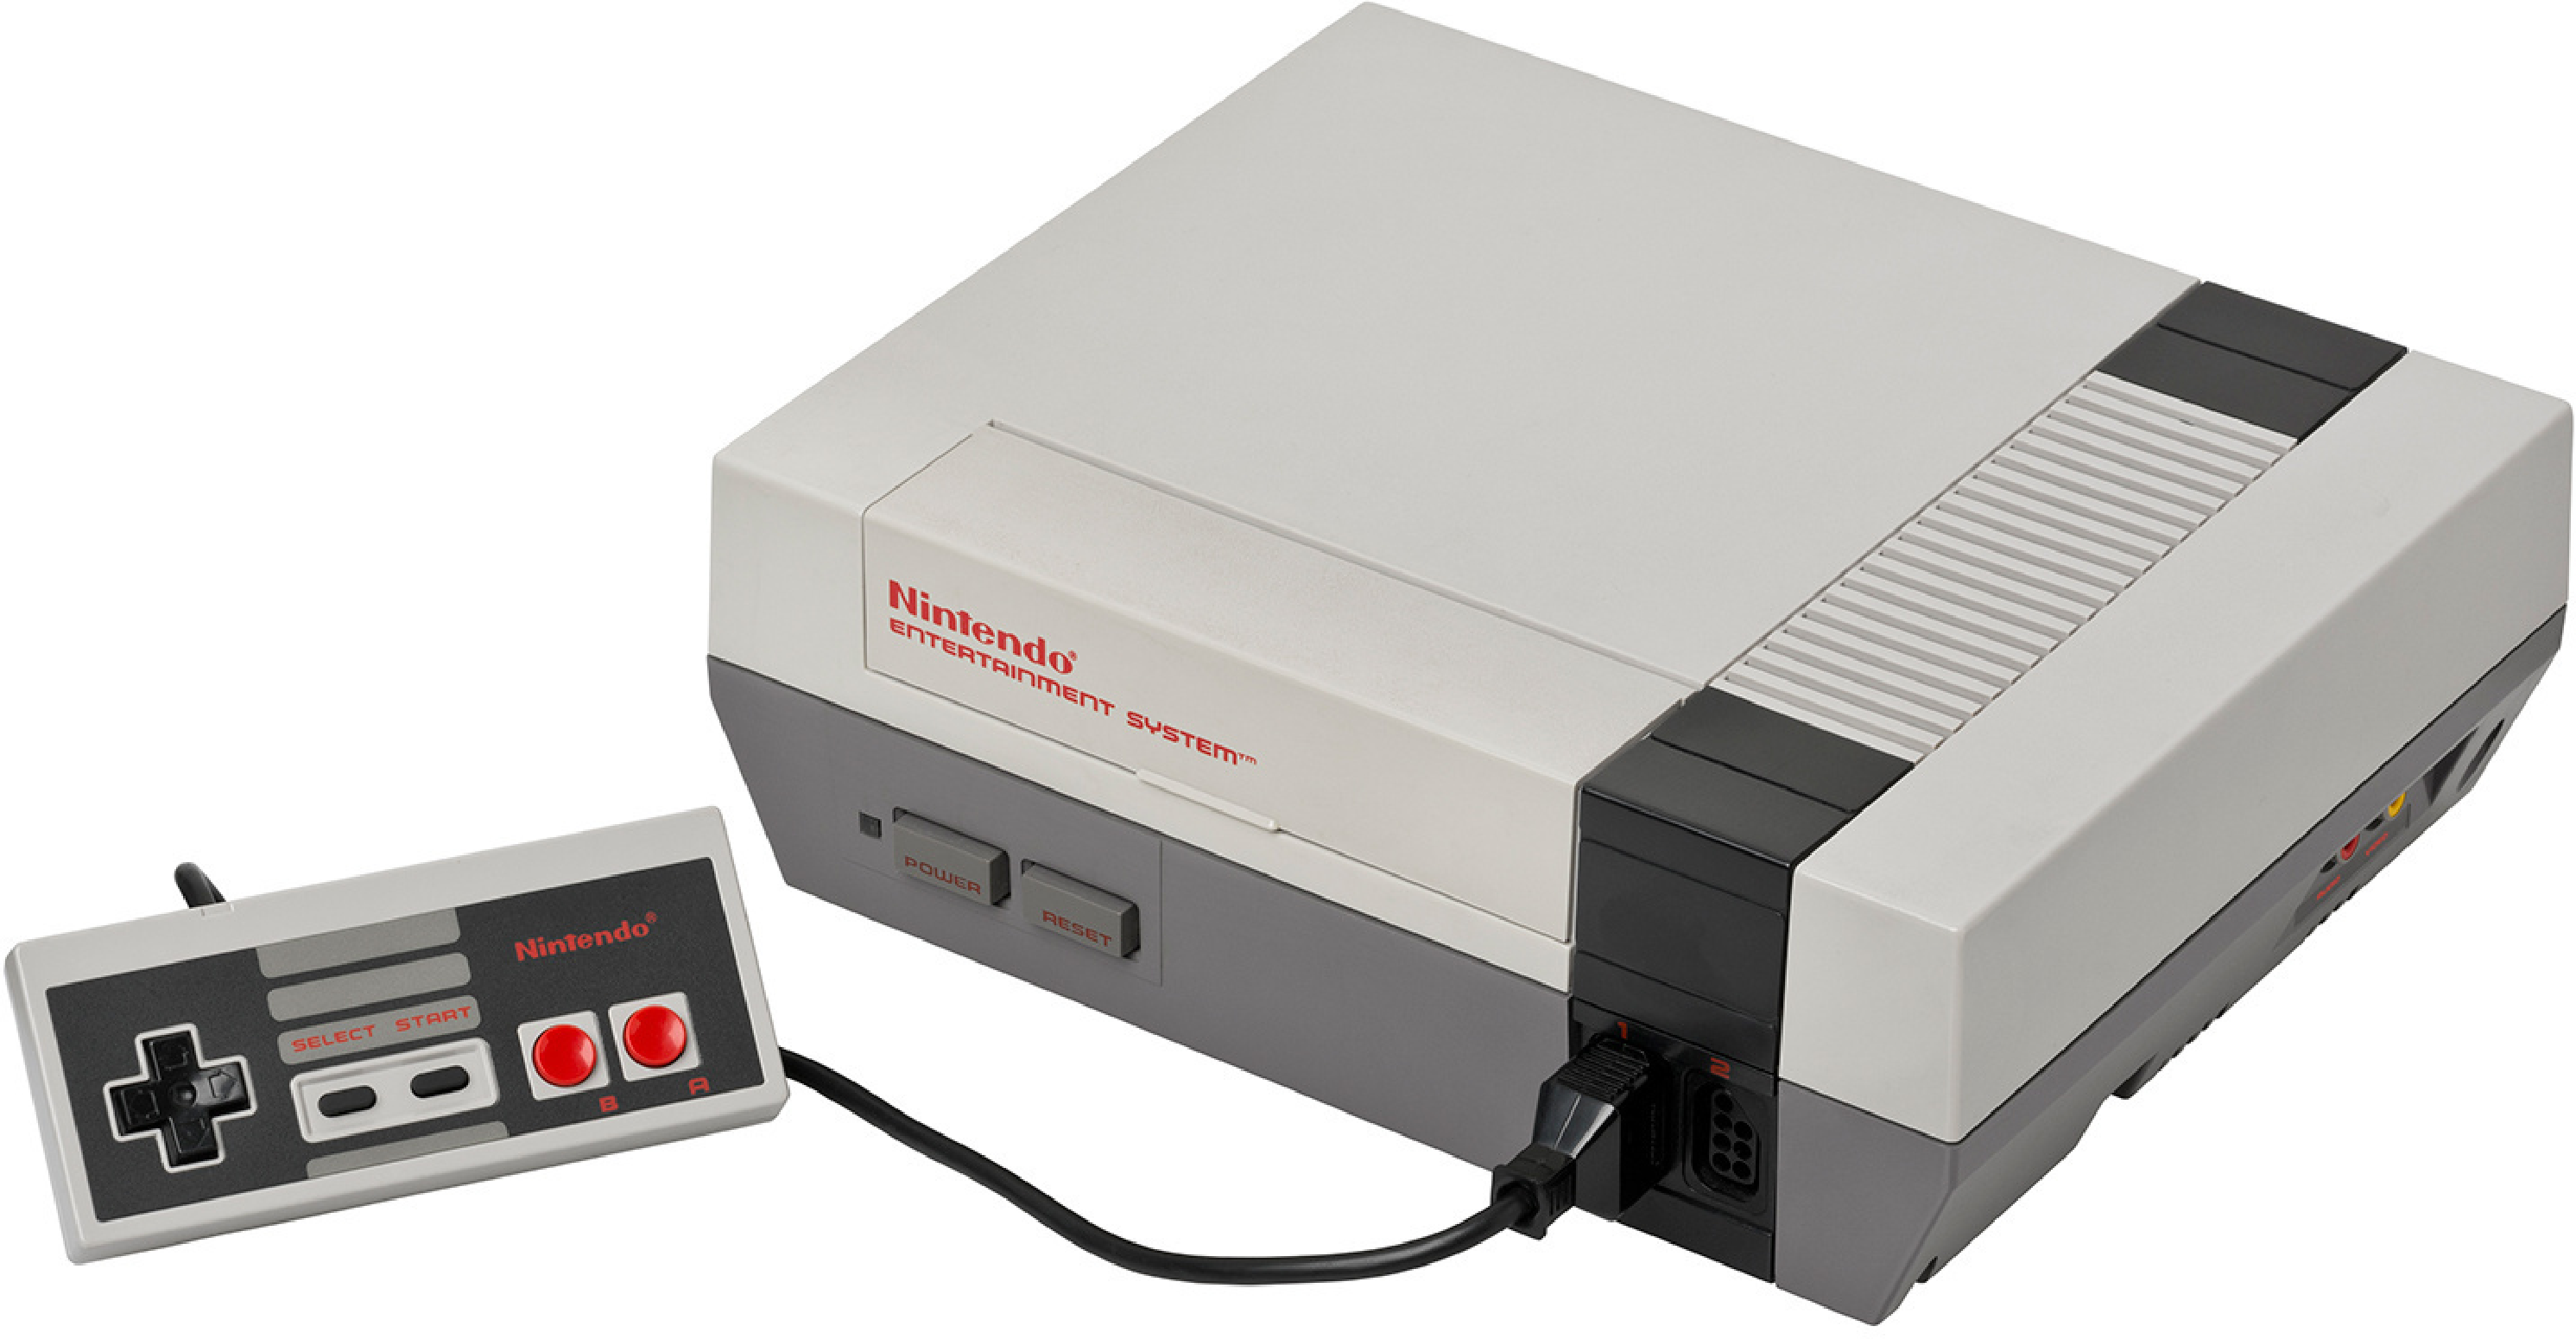
\includegraphics[height=70pt]{figures/nintendo-classic}
		\qquad
		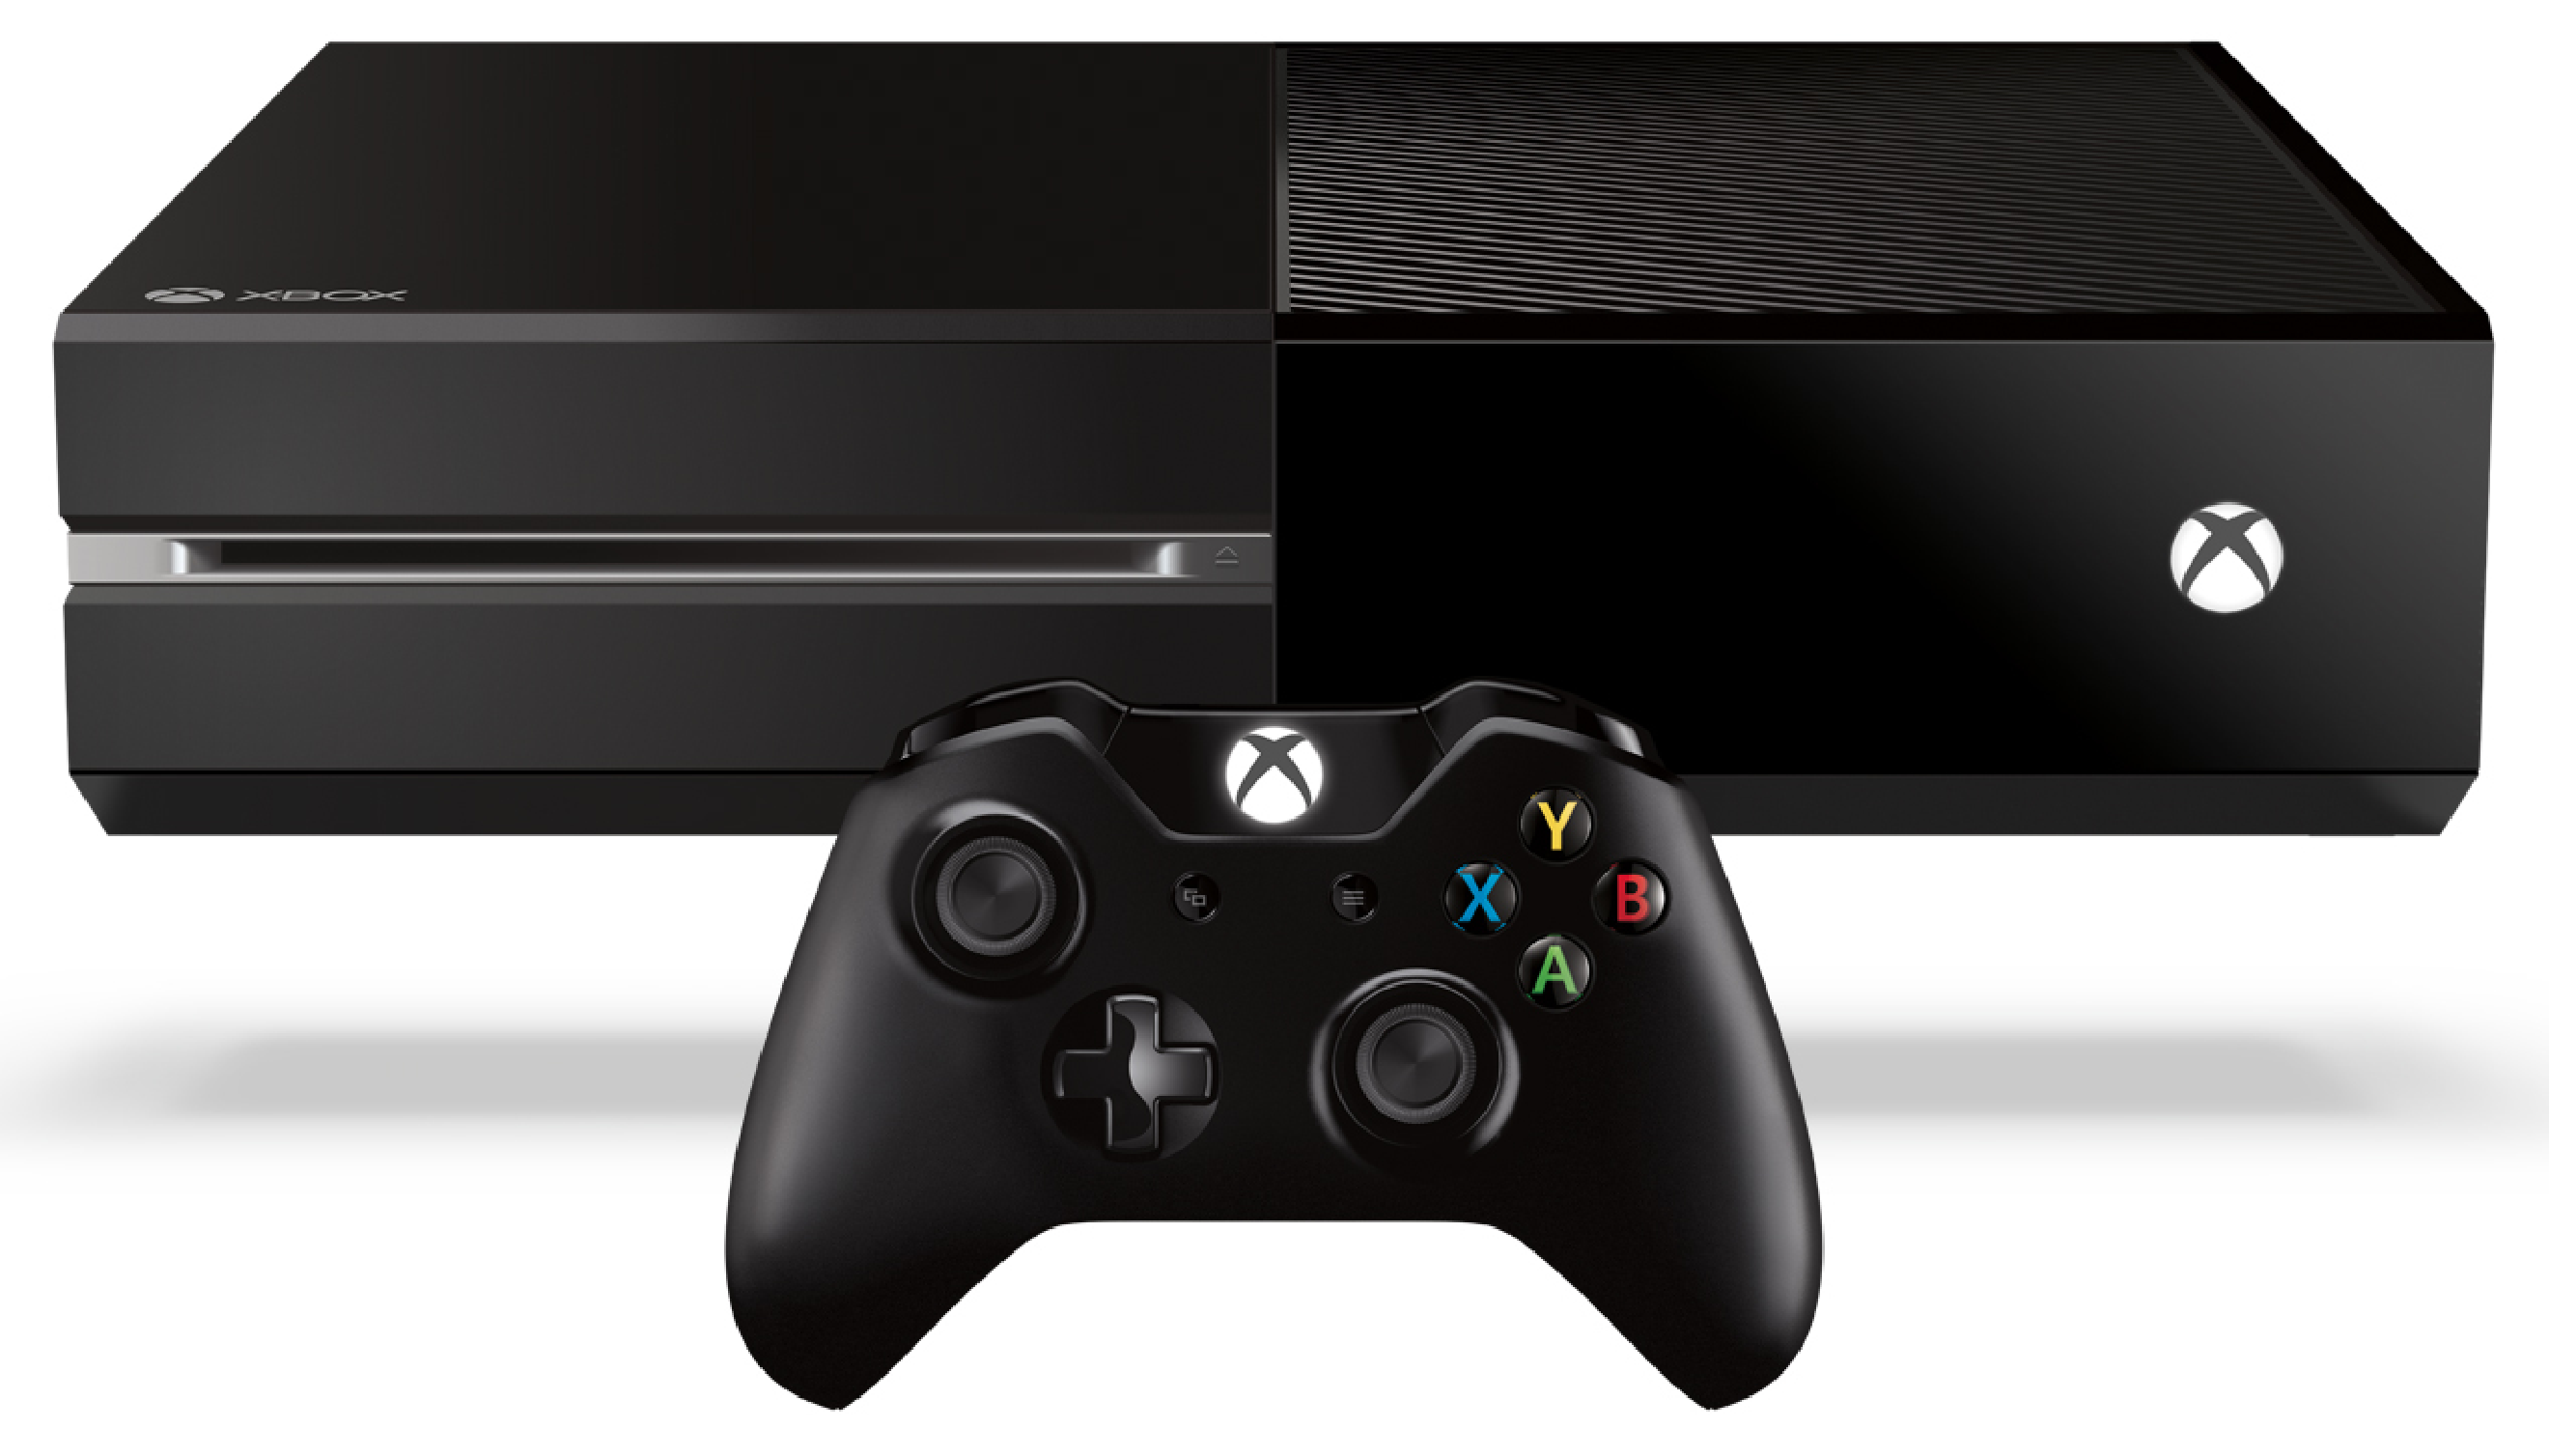
\includegraphics[height=70pt]{figures/xbox-one}
	\end{figure}
}

\end{frame}

\begin{frame}
\frametitle{Architecture Description Languages}

ADLs are useful tools for systems development. They let us:
\begin{itemize}
	\item<2-> ...describe systems at different levels of abstraction
%	\begin{itemize}
%		\item<2-> At a low level, for cycle-accurate simulation
%		\item<2-> At a high level, for rapid prototyping
%	\end{itemize}
	\item<3-> ...use new technologies without rewriting all of our tools
	\item<4-> ...separate the behaviour of tools from their implementation
\end{itemize}

\end{frame}

\begin{frame}
\frametitle{Architecture Description Languages}

We consider ADLs mostly in the context of simulation
\begin{itemize}
	\item Low level ADLs are more suited to detailed simulation
	\item More abstract ADLs are better suited to fast simulation
\end{itemize}

\end{frame}
